 \newpage

\section{La Oferta, la Demanda y la Política Económica}

\subsection{Controles de Precios}
Si el mercado se regula de manera eficiente de formula autonoma. Cuál es la necesidad de tener agentes politicos que creen restricciones ?
Por lo general esta arbitrariedad se da cuando se considera injusto el precio acordado en equilibrio.
\subsection{Precio Maximo}
\subsection{Precio Minimo}

\subsection{Controlar sin controlar}
Cuando Se crea una legislacion que no influye sobre el mercado. a continuacion dos ejemplos de como se pueden crear politicas sin influencia en el mercado 
\begin{center}
	\begin{figure}[h]
		\centering
		\begin{subfigure}	
			\left
			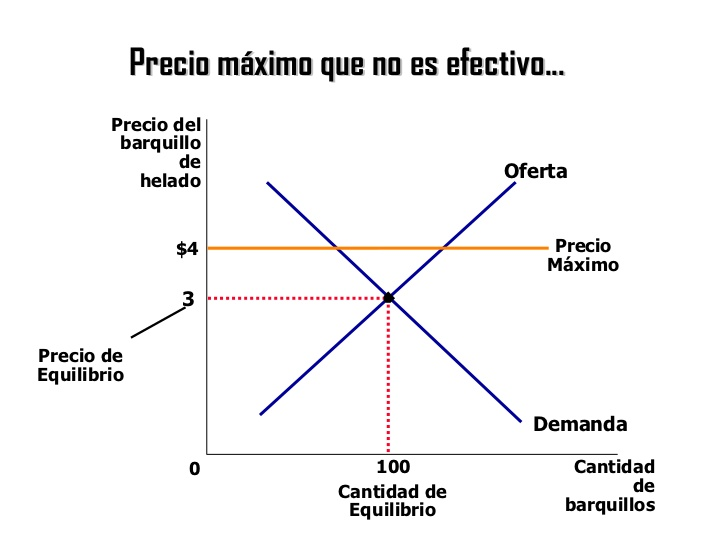
\includegraphics[scale=0.3]{images/61.jpg}
		\end{subfigure} 	
		\begin{subfigure}
			\left	
			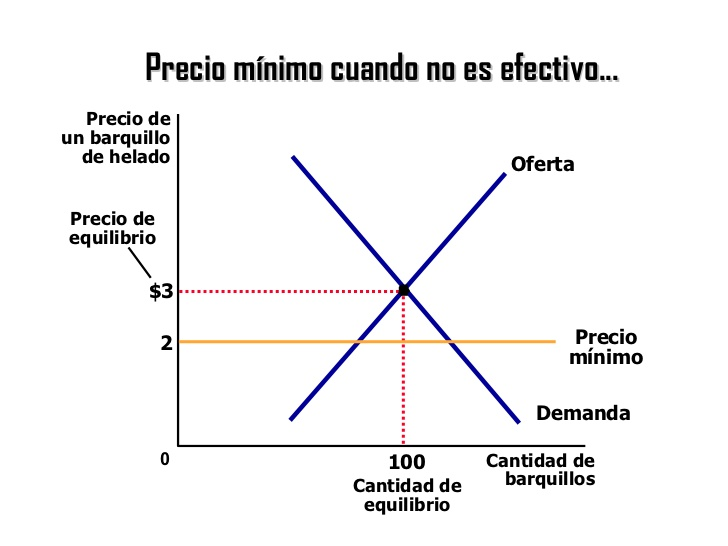
\includegraphics[scale=0.3]{images/62.jpg}
		\end{subfigure} 
		\begin{subfigure}
		\left	
		\includegraphics[scale=0.3]{images/meme3.jpg}
	\end{subfigure} 		
	\end{figure}
\end{center}